\begin{frame}{Утилитаризм}
    \begin{columns}[T,onlytextwidth]
        \begin{column}{0.56\textwidth}
            \begin{itemize}
                \item<1-> Утилитаризм --- получение пользы практического толка через удовлетворение своих потребностей
                \item<2-> Художественные формы и образы стали приобретать практическое значение
                \item<3-> Если рисунок, то для ткани, фотография стала использоваться в
                фотомонтаже и коллаже в журналах и рекламных плакатах и т.д.
            \end{itemize}
        \end{column}
        \begin{column}{0.4\textwidth}
            \visible<2->{
                \begin{figure}
                    \centering
                    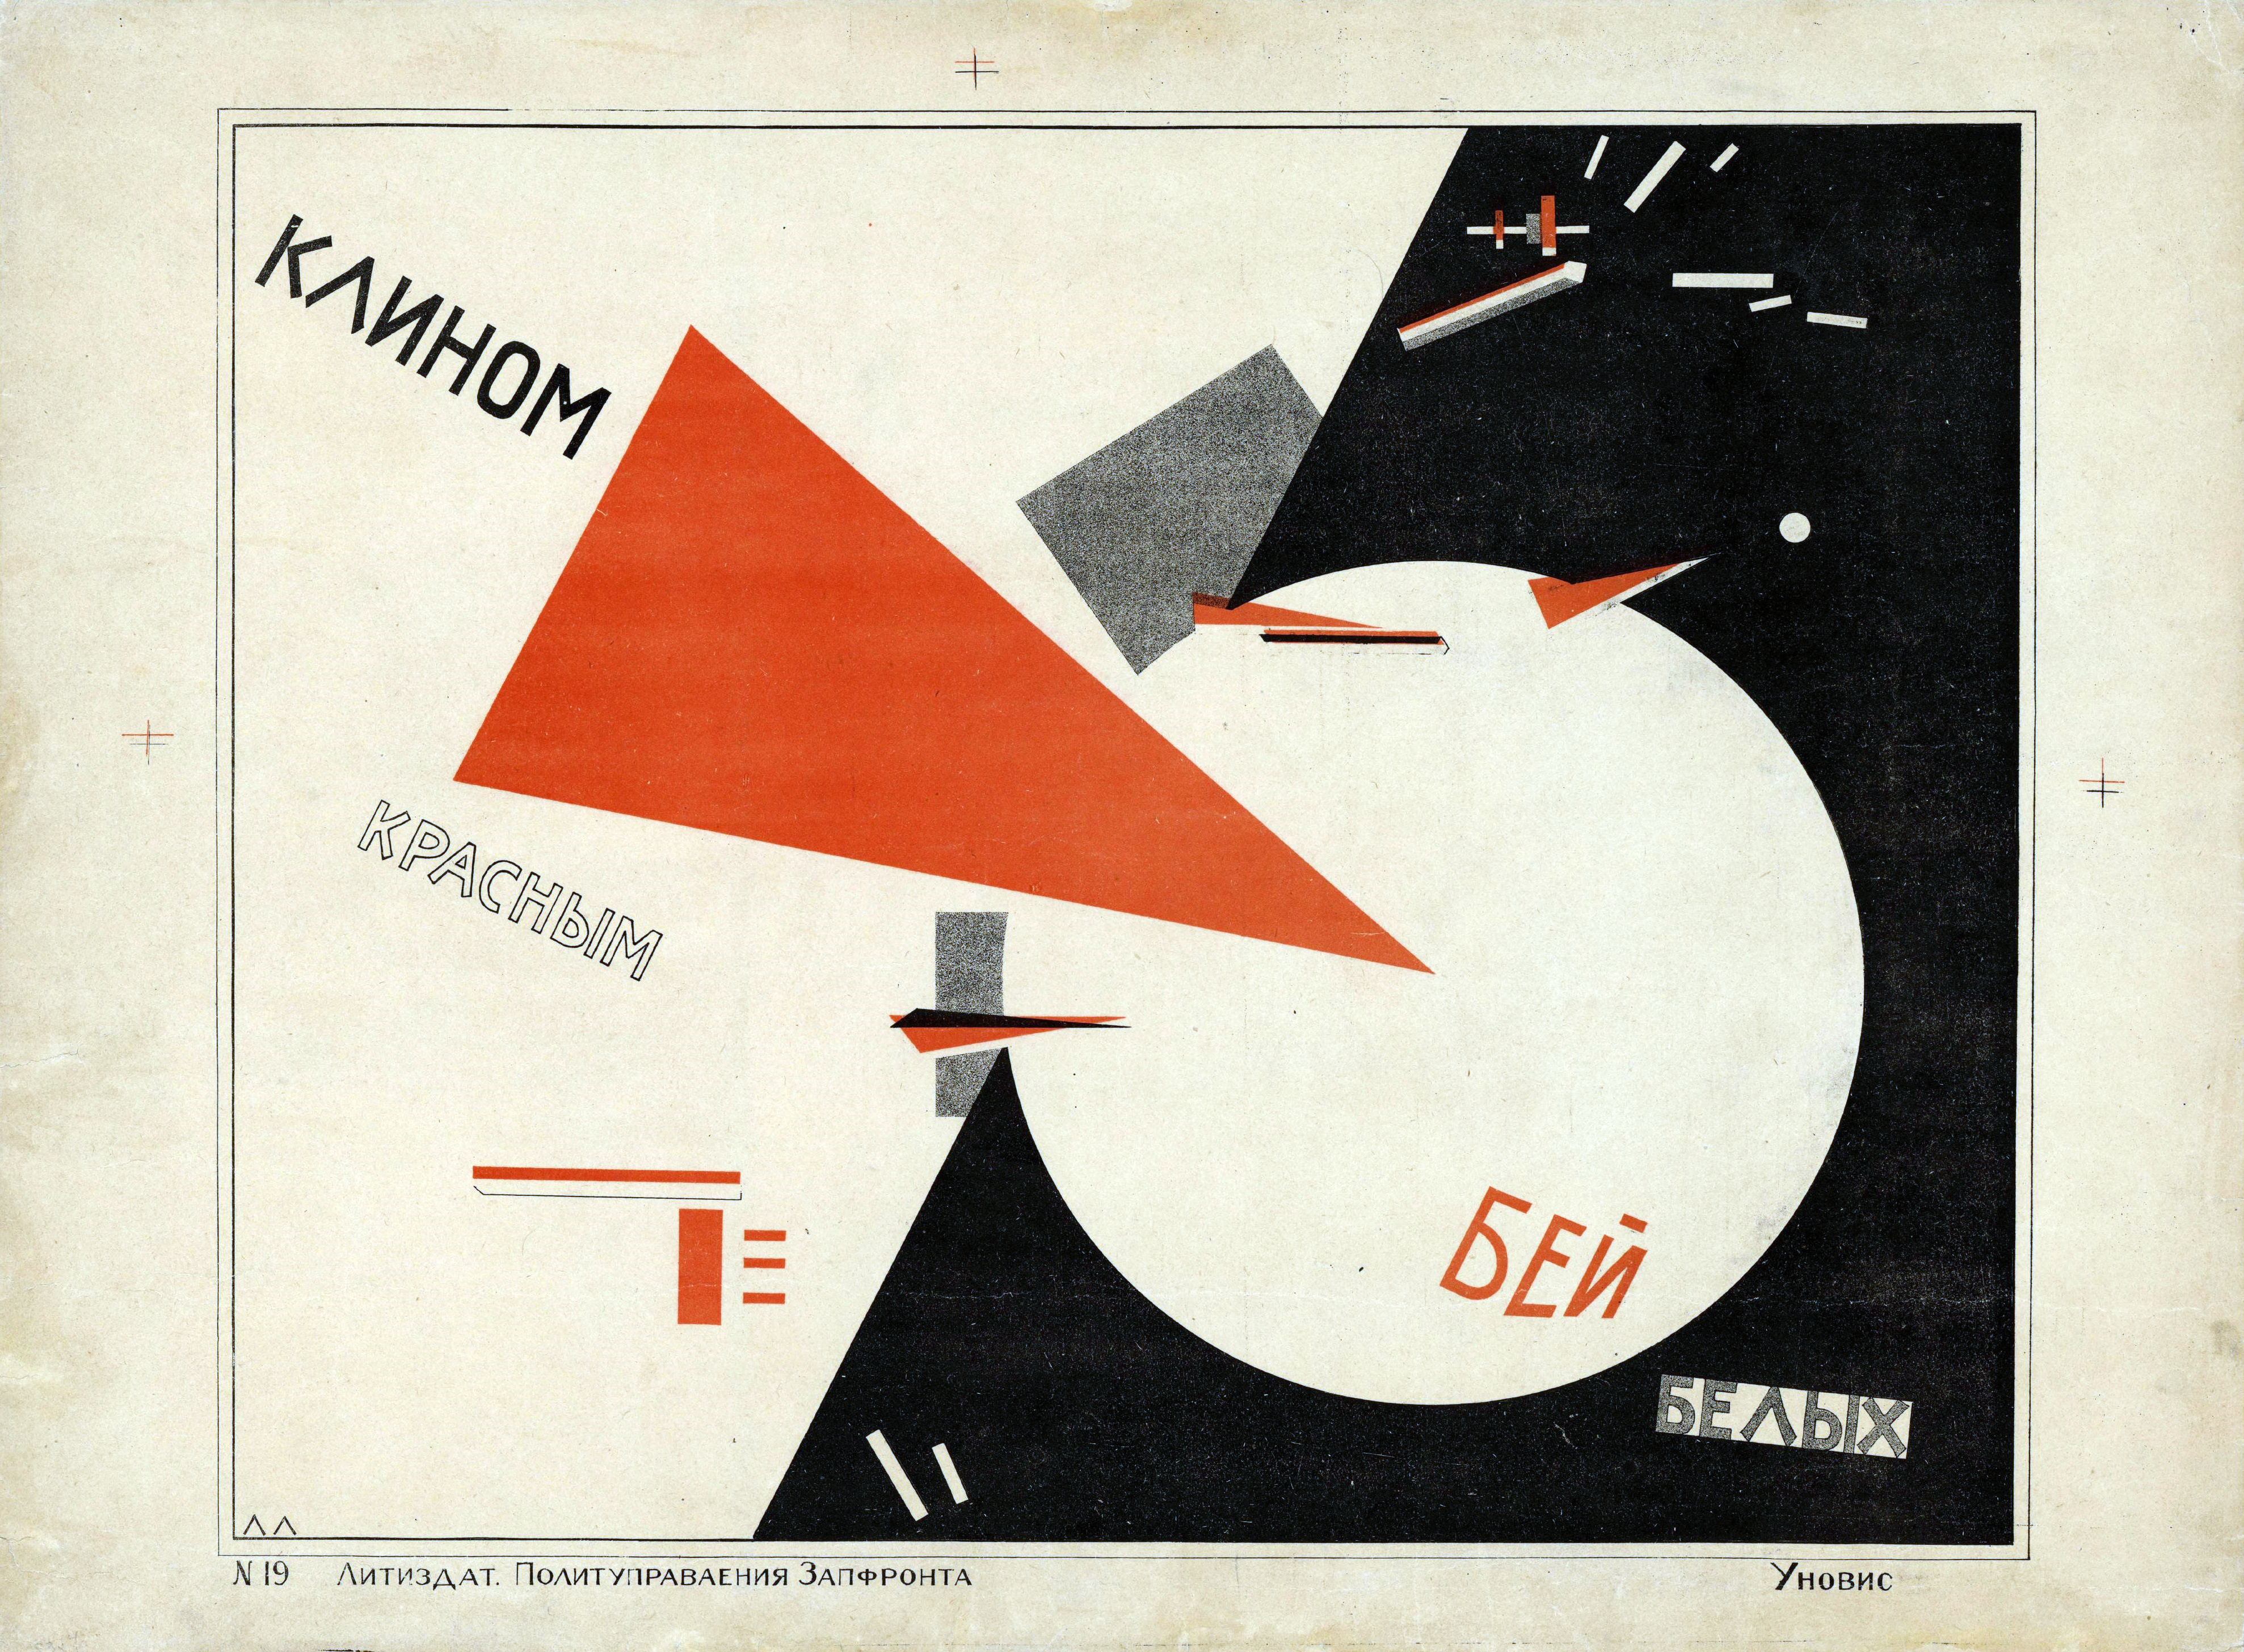
\includegraphics[width=\textwidth]{images/Klinom_Krasnym_Bej_Belych.jpg}
                    \caption*{<<Клином красным бей белый>> \\ Эль Лисицкий, 1920 г.}
                \end{figure}
            }
        \end{column}
    \end{columns}

\end{frame}